
\section{Waarom een PWA}

In dit onderdeel van de literatuurstudie zal er onderzocht worden wat de redenen zijn om een PWA te ontwikkelen voor een project. De voordelen zullen bekeken worden in vergelijking met traditionele webapplicaties en native applicaties.
\autocite{TandelSunil2018}


\subsection{Bereik}
	Volgens Google heeft Google Chrome meer dan 1 miljard mobiele gebruikers. In 2016 was dit nog maar 400 miljoen. Steeds meer mensen gebruiken hun smartphone om op zoek te gaan naar informatie. 
	\autocite{Nath2017}
	
	Data toont aan dat gebruikers nog steeds 87\% van hun tijd op hun smartphone spenderen in native applicaties. Van deze 87\% wordt 80\% van de tijd in slechts 3 verschillende applicaties gespendeerd. Terwijl er veel tijd besteed wordt in native applicaties, is het toch heel moeilijk om tijd te krijgen van de gebruiker om jouw applicatie te gebruiken.
	
	De acquisitie is bij het web groter dan bij native applicaties. De gemiddelde gebruiker download 0 nieuwe applicaties per maand. 
	
	Op het web, waar slechts 13\% van de tijd van de mobiele gebruikers besteed wordt, worden er echter maandelijks ongeveer 100 websites bezocht. Hier is er voor bedrijven dus een kans om een gebruiker jouw platform te laten ontdekken en nieuwe gebruikers te winnen.
	\autocite{GoogleChromeDevelopers2017}
	

\subsection{Platformonafhankelijkheid }
	Een van de grootste voordelen van het web is dat het platformonafhankelijk is. Een webapplicatie hoeft maar eenmaal ontwikkeld te worden en kan dan op meerdere platformen gebruikt worden. Het web is ook niet gebonden aan deze conventionele platformen. De dag van vandaag zijn meer en meer toestellen zoals televisies, game-consoles en e-readers verbonden met het internet. 
	
	PWA's kunnen meer complexe functionaliteiten implementeren dan een traditionele webapplicatie. Bepaalde functionaliteiten zijn wel platformafhankelijk. Een functionaliteit die kan toegevoegd worden is push notificaties. Zoals aangetoond in vorig hoofdstuk zal dit niet werken op iOS-toestellen. De PWA zal wel nog werken op iOS maar zal niet genieten van deze functionaliteit. PWA's zijn dus gedeeltelijk platformonafhankelijk.
	
	Bij native ontwikkeling zijn er vaak verschillende codebases voor elk platform die het ondersteunt. Er zijn technologieën die dit proberen op te lossen zoals React Native. Maar ook hier moet er voor bepaalde delen nog native code geschreven worden per platform. Native applicaties zijn dus niet platformonafhankelijk. 
	
	Thomas Steiner maakte in een interview ook duidelijk dat de 'Build once, run everywhere' een grote troef is voor PWA's.
	(appendix~\ref{ch:Interview})

\subsection{Omzet}
	Conversion rate is een meeteenheid die gebruikt wordt om de omzet van een website te peilen. Hoe hoger de conversion rate hoe beter. De conversion rate wordt bepaald door het aantal ‘conversions’ die een website heeft ten opzichte van het aantal bezoekers. Een conversion kan voor elke website anders gedefinieerd worden. Voor een e-commerce website zal dit vaak een aankoop zijn. Voor andere websites kan dit het aanmelden van de gebruiker op de nieuwsbrief zijn.
	\autocite{GoogleSupport2020}
	
	Nikkei is een nieuws-website die in 2018 zijn website ombouwde tot een PWA.  Door het gebruik van service workers konden ze de laadtijd van hun website drastisch verlagen (14 seconden sneller:  van \SI{\pm 20} seconden naar  \SI{\pm 6} seconden). Dit had als gevolg dat gebruikers steeds vaker naar Nikkei gingen als nieuwsbron. 
	
	De conversion rate steeg met 58\% (premium abonnement) en er was een stijging van 49\% in het aantal dagelijkse gebruikers. Deze gebruikers lazen gemiddeld het dubbel aantal artikelen dan voordien. 
	\autocite{Developers2018}
	
	Dit voorbeeld toont aan dat de omzet met een PWA hoger kan zijn dan bij traditionele webapplicaties.
	
	Met native applicaties kan er nog steeds een meer gepersonaliseerde ervaring geboden worden en zal er gemiddeld gezien ook een hogere conversion rate zijn. Maar PWA's scoren beter dan traditionele websites.
	\autocite{Anastasia2019}
	

\subsection{Bundle size}
\begin{center}

\end{center}
	Bundle size is de grootte van de applicatie als deze geïnstalleerd wordt. Het is positief om een zo klein mogelijke bundle size te hebben. \autocite{Scott2019}
	
	Tinder besliste om zijn service ook aan te bieden als een PWA. Tinder slaagde erin om alle functionaliteiten die hun native applicaties hebben over te nemen in de PWA. Ze slaagden hierin door gebruik te maken van verschillende web API's. 
	\autocite{Osmani2017}
	
	Eén van de grootste voordelen is dat de PWA (versie 118) op het moment van schrijven slechts een grootte heeft van 397KB. De native Android applicatie (versie 11.8.1) daarentegen neemt 130MB in beslag op een toestel.
	
	In Westerse landen is dit handig, maar zal het niet snel bepalen of een gebruiker een applicatie effectief gebruikt. In andere markten zoals Afrika is dit heel belangrijk. De toestellen die er gebruikt worden, zijn vaak verouderd en hebben mindere specificaties dan de toestellen gebruikt in het Westen. 
	
	De gemiddelde prijs van de top 5 meest verkochte smartphones in Afrika was 135,6 USD. Deze toestellen beschikken vaak over slechts 8 of 16GB opslagruimte. 
	\autocite{netAdmin2017}
	
	Slechts 7\% van de Afrikaanse bevolking beschikt over een 4g-connectie. De andere gebieden moeten het vaak doen met een tragere 3g-connectie.	
	\autocite{gsmArena2020}

	In deze markten is het dus cruciaal om zo klein mogelijke applicaties te leveren.
	
	\begin{figure}[H]
		\centering
		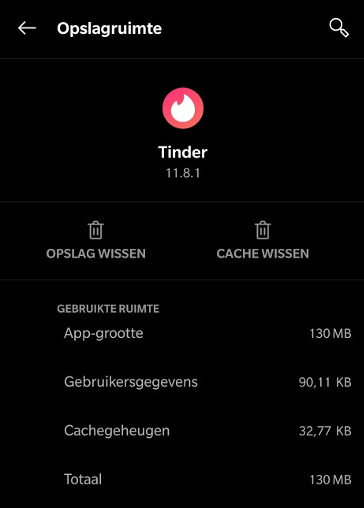
\includegraphics{./img/tinder_native.png}
		\caption{Tinder voor Android -  versie 11.8.1}
	\end{figure}
	
	\begin{figure}[H]
		\centering
		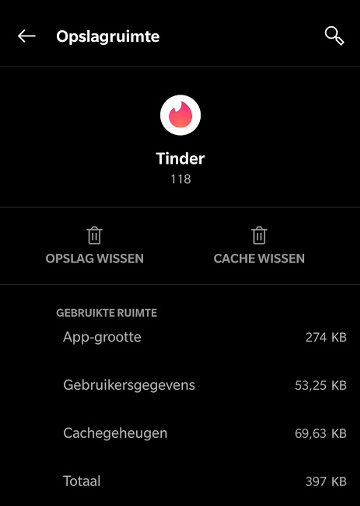
\includegraphics{./img/tinder_pwa.png}
		\caption{PWA-versie 118}
	\end{figure}

\subsection{Offline gebruik}
	Een webapplicatie kan nu geïmplementeerd worden met een ‘offline-first’ benadering. Offline first is gelijkaardig aan progressive enhancement. Eerst wordt er een applicatie gebouwd die volledig offline beschikbaar is, die vervolgens uitgebreid wordt met online functionaliteiten. 
	
	Door gebruik te maken van de fetch API in een service worker kunnen API-calls onderschept worden. De service worker kan vervolgens controleren of de gebruiker online is. Als dit niet het geval is, kan de service worker de API-call annuleren en zelf een antwoord sturen met een 200-status en een melding dat er geen internet is. Op basis hiervan kan er een gepaste boodschap getoond worden aan de gebruiker en zal de applicatie niet crashen.
	\autocite{Developers2019a}
	
	Data van API-calls kan ook lokaal opgeslagen worden. Als een bepaalde API-call herhaald wordt, kan in plaats van de backend aan te spreken de lokale data gebruikt worden. Dit zal de ervaring voor gebruikers met een zwakke of inconsistente netwerk-connectie verbeteren.
	\autocite{Vanhala2017}
	
	
\subsection{Betrokkenheid}
	Een van de redenen om een native applicatie te maken, was vaak betrokkenheid. Via het web heb je een groot bereik, maar gebruikers op een bepaald platform houden was moeilijk. Push notificaties kunnen hier een oplossing voor bieden.
	\autocite{Google2019}

	Push notificaties zijn meldingen die op het toestel van een gebruiker tevoorschijn komen. Deze worden verstuurd van een server en zijn dus niet afhankelijk van input van een gebruiker. Door gebruik te maken van de Push API en de Notifications API kunnen deze meldingen gebruikt worden bij een PWA.
	
	Push notificaties kunnen gebruikers er aan herinneren om een bepaalde applicatie terug te gebruiken. 
	\autocite{Hiltunen2018}
	
	Push notificaties kunnen ook gebruikt worden om de conversion rate te verhogen. Bijvoorbeeld bij een e-commerce platform kan er een melding gestuurd worden als de klant items in zijn mandje heeft geplaatst maar deze nog niet heeft besteld.
	\autocite{Gaunt2020}

	Als een webapplicatie voldoet aan de criteria (zie hoofdstuk \ref{ch: Wat is een PWA}) van een PWA, kan deze toegevoegd worden aan het startscherm van een toestel. Hierdoor wordt het voor de gebruiker gemakkelijker om een PWA herhaaldelijk te gebruiken. Als een applicatie wordt geopend vanaf het startscherm, kan deze het volledige scherm gebruiken en zullen adresbalk en andere tools van de browser weggelaten worden. Dit zorgt ervoor dat de PWA meer zal aanvoelen als een native applicatie dan een website.
	
	Door deze nieuwe functionaliteiten toe te voegen, is de betrokkenheid van een PWA groter dan die van een traditionele webapplicatie. Nog niet alle functies die beschikbaar zijn voor native applicaties zijn beschikbaar voor PWA's.
	

\subsection{Kost}
	Het ontwikkelen van native applicaties is niet goedkoop. Services zoals Spotify moeten native applicaties ontwikkelen voor verschillende platformen (macOS, Windows, iOS, Android, Linux, ChromeOS).
	
	Het creëren van een digitaal product voor verschillende platformen is vaak te duur voor een kleiner of startend bedrijf. Progressive Web Apps kunnen hier een oplossing bieden. Een PWA kan geïnstalleerd worden op al de bovenstaande platformen. In plaats van eenzelfde applicatie te bouwen voor verschillende platformen, kan er met PWA's dus één applicatie geschreven worden die op verschillende platformen kan gebruikt worden.
	
	Spotify implementeerde zijn service ook als een PWA. \autocite{Spotify2020} Al de functies die op de native applicaties beschikbaar zijn, zijn ook beschikbaar via deze webapplicatie. Enkel de offlinefunctie is (nog) niet geïmplementeerd. Ook het gebruik van de functietoetsen op het toetsenbord van een desktop is niet ondersteund.
	\autocite{Vu2019}
	
	
\subsection{Deployment}

	Het uitgeven van een PWA is ook een stuk gemakkelijker en goedkoper dan het verdelen van native applicaties via de verschillende app-stores. 
	Om een applicatie te publiceren in de Apple app-store moet de ontwikkelaar een “Apple developer” account hebben. Dit kost 99 euro per jaar. 
	\autocite{Apple2020b}
	
	Ook het publiceren van een applicatie op de Google Play Store is niet gratis. De uitgever moet een developer account hebben bij Google Play. Dit kost eenmalig 25 euro.
	Elke app-store (Windows, Apple, Android, Chrome, …) heeft zijn eigen specifieke eisen en kosten om een applicatie te kunnen uploaden. Bij een PWA hoeft er slechts één applicatie online gezet te worden. Deze moet niet gevalideerd worden door andere partijen. 
	\autocite{GooglePlay2020}
	
	Het publiceren van een applicatie op de Windows store is gratis.
	
	Het publiceren van een PWA is meestal ook niet gratis. Het online brengen van een website heeft meestal 2 kosten: enerzijds de aankoop van een domein en anderzijds de hosting van een applicatie met HTTPS-verbinding. Deze kosten zijn ook nodig bij traditionele webapplicaties.
	Een domein aankopen via de website versio.nl kost 28,95 euro voor vijf jaar.
	\autocite{Versio2020}
	
	Het hosten van een statische applicatie kan via bepaalde platformen kosteloos gebeuren. Voorbeelden van deze platformen zijn \href{https://firebase.google.com/}{Firebase} en \href{https://www.netlify.com/}{Netlify}	
	Deze platformen bieden ook gratis SSL-certificaten aan zodat er een HTTPS-connectie is. 
	
	De kost om een PWA online te brengen is dus even hoog als bij traditionele websites. De kost is wel lager dan bij native applicaties. 	
	
	De kost is niet het enige voordeel van het online brengen van PWA's ten opzichte van native applicaties. Als een applicatie gepubliceerd wordt in de Apple App store of in de Google Play Store, dan moeten deze voldoen aan een groot aantal richtlijnen. Bij het uploaden van een applicatie wordt deze eerst gecontroleerd door Apple en Google of deze wel voldoet aan deze richtlijnen. 
	\autocite{Apple2020c}
	\autocite{GooglePlay2020a}
	
	Dit betekent dus dat niet elke applicatie gepubliceerd kan worden in deze app-stores. Een PWA moet niet gevalideerd worden door een overkoepelend bedrijf. Elke applicatie die de ontwikkelaar maakt, kan dus gepubliceerd worden.
	Een ander gevolg is dat het gemiddeld 72 uur duurt om een app te laten valideren door beide app-stores. Dit is slechts een gemiddelde, want dit kan uitlopen tot een week en langer.
	\autocite{Siddiqui2019}
	
	Dit is een vertraging die webapplicaties en PWA's niet hebben.
	
	Uit het interview met zowel Thomas Steiner als bij Wassim Chegham blijkt dat het onafhankelijk zijn van een app-store een grote meerwaarde is. Ze haalden beiden aan dat de iOS waarmee een PWA gehost en geüpdatet kan worden een uniek voordeel is.
	(appendix~\ref{ch:Interview})
	
\subsection{Updates}

	Als een PWA bezocht wordt, zal deze steeds de meeste recente versie tonen. Als er een update moet gebeuren, kan de ontwikkelaar kiezen om dit wel of niet aan de gebruiker te laten weten. 	
	\autocite{Hume2018}
	
	Kleinere updates die de gebruiker niet zal opmerken kunnen uitgevoerd worden zonder dat de gebruiker dit weet.
	 \autocite{Sanderson2020}
	 
	Als er grotere updates zijn, is het een betere user experience om de gebruiker te informeren dat er een update zal uitgevoerd worden.
	\autocite{Wicki2017}
	 
	De ontwikkelaar heeft dus volledige vrijheid in hoe hij omgaat met updates. De gebruiker kan steeds genieten van de laatste versie van de applicatie zonder dat hij deze zelf manueel moet updaten. Deze ervaring is dezelfde voor traditionele websites.
	
	Zowel Android als iOS hebben een functionaliteit om hun applicaties automatisch te updaten. Deze functionaliteit werkt echter enkel voor kleine incrementele updates. Als de applicatie functionaliteiten aanpast, toevoegt of verwijdert, moet deze app nog steeds manueel geüpdatet worden via de app-store. Als ontwikkelaar heb je dus geen controle over welke versie de gebruiker aan het gebruiken is.
	\autocite{Apple2020d}
	\autocite{AndroidDevelopers2020}
		

\subsection{Conclusie}
	\begin{table}[H]
		\centering
		\begin{tabular}{llll}
			                         			  & Web applicatie 	 				 & PWA								 & Native applicatie \\
			Bereik                   		   & \cellcolor{green!40}      		 & \cellcolor{green!40}			& \cellcolor{red!50}\\
			Platformonafhankelijkheid   & \cellcolor{green!40}      	  & \cellcolor{orange!50}		& \cellcolor{red!50}\\
			Omzet   						  & \cellcolor{red!50}      		 & \cellcolor{orange!50}		& \cellcolor{green!40}\\
			Bundle size						  & niet van toepassing      		& \cellcolor{green!40}		   & \cellcolor{red!50}\\
			Offline gebruik					 & \cellcolor{red!50}      		    & \cellcolor{green!40}			& \cellcolor{green!40}\\
			Betrokkenheid 					& \cellcolor{red!50}      		   & \cellcolor{orange!50}		 & \cellcolor{green!40}\\
			Kost 								& niet van toepassing     		  & \cellcolor{green!40}		 & \cellcolor{red!50}\\
			Deployment 						& \cellcolor{green!40}      	  & \cellcolor{green!40}		 & \cellcolor{red!50}\\
			Updates	   						& \cellcolor{green!40}      	  & \cellcolor{green!40}		 & \cellcolor{red!50}\\
		\end{tabular}
		\caption{concluderende tabel 'waarom een PWA'}
	\end{table}
	
	\begin{table}[H]
		\centering
		\begin{tabular}{lll}
			Positief \cellcolor{green!40} & Matig \cellcolor{orange!50} & Negatief  \cellcolor{red!50}
		\end{tabular}
	\end{table}
	
	
